\section{Simulation}

\subsection{Testbench Architecture}

The professional testbench is organized into independent task-based test cases, each with its own reset sequence to ensure test isolation and reproducibility. The testbench is structured as follows:

\begin{itemize}
    \item \textbf{System Clock}: 5 kHz (CLK\_PERIOD = 200,000 ns)
    \item \textbf{LED Configuration}: 16 LEDs with 12 clockwise steps and 8 anti-clockwise steps
    \item \textbf{Timing}: TimeStep parameter set to 500 ms per state transition
    \item \textbf{Task-Based Design}: Each test case is implemented as an independent task that applies its own reset before executing its test scenario
\end{itemize}

\subsection{Test Cases and Functional Verification}

\subsubsection{TC1: Normal Operation (Legacy Baseline)}

\textbf{Objective}: Verify normal ring flasher operation with continuous repetition followed by controlled fade-out.

\textbf{Test Flow}:
\begin{enumerate}
    \item Apply reset: hold \texttt{reset = 1} for 10 clock cycles
    \item Release reset: set \texttt{reset = 0} and wait 100 cycles for system settlement
    \item Activate sequence: set \texttt{rep = 1} and run for $40 \times \text{CLK\_FREQ}$ cycles ($\approx 8$ seconds at 5 kHz)
    \item Deactivate sequence: set \texttt{rep = 0} and run for $5 \times \text{CLK\_FREQ}$ cycles ($\approx 1$ second) to observe fade-out
\end{enumerate}

\textbf{Expected Behavior}:
\begin{itemize}
    \item While \texttt{rep = 1}: CW motion for exactly 12 steps with LED incrementing positions, then ACW motion for exactly 8 steps with LED decrementing positions
    \item Pattern repeats continuously while \texttt{rep = 1}
    \item Upon \texttt{rep = 0}: FSM completes the current CW or ACW cycle before entering OFF\_STATE (no immediate stop)
    \item After current cycle completes: LEDs gradually fade as brightness levels decrement on each \texttt{divclk} pulse
    \item When all LED brightness levels reach zero: \texttt{off\_all} signal triggers and FSM transitions back to IDLE\_STATE
    \item All control signals synchronized to \texttt{divclk} at 500 ms intervals
\end{itemize}

\begin{figure}[H]
    \centering
    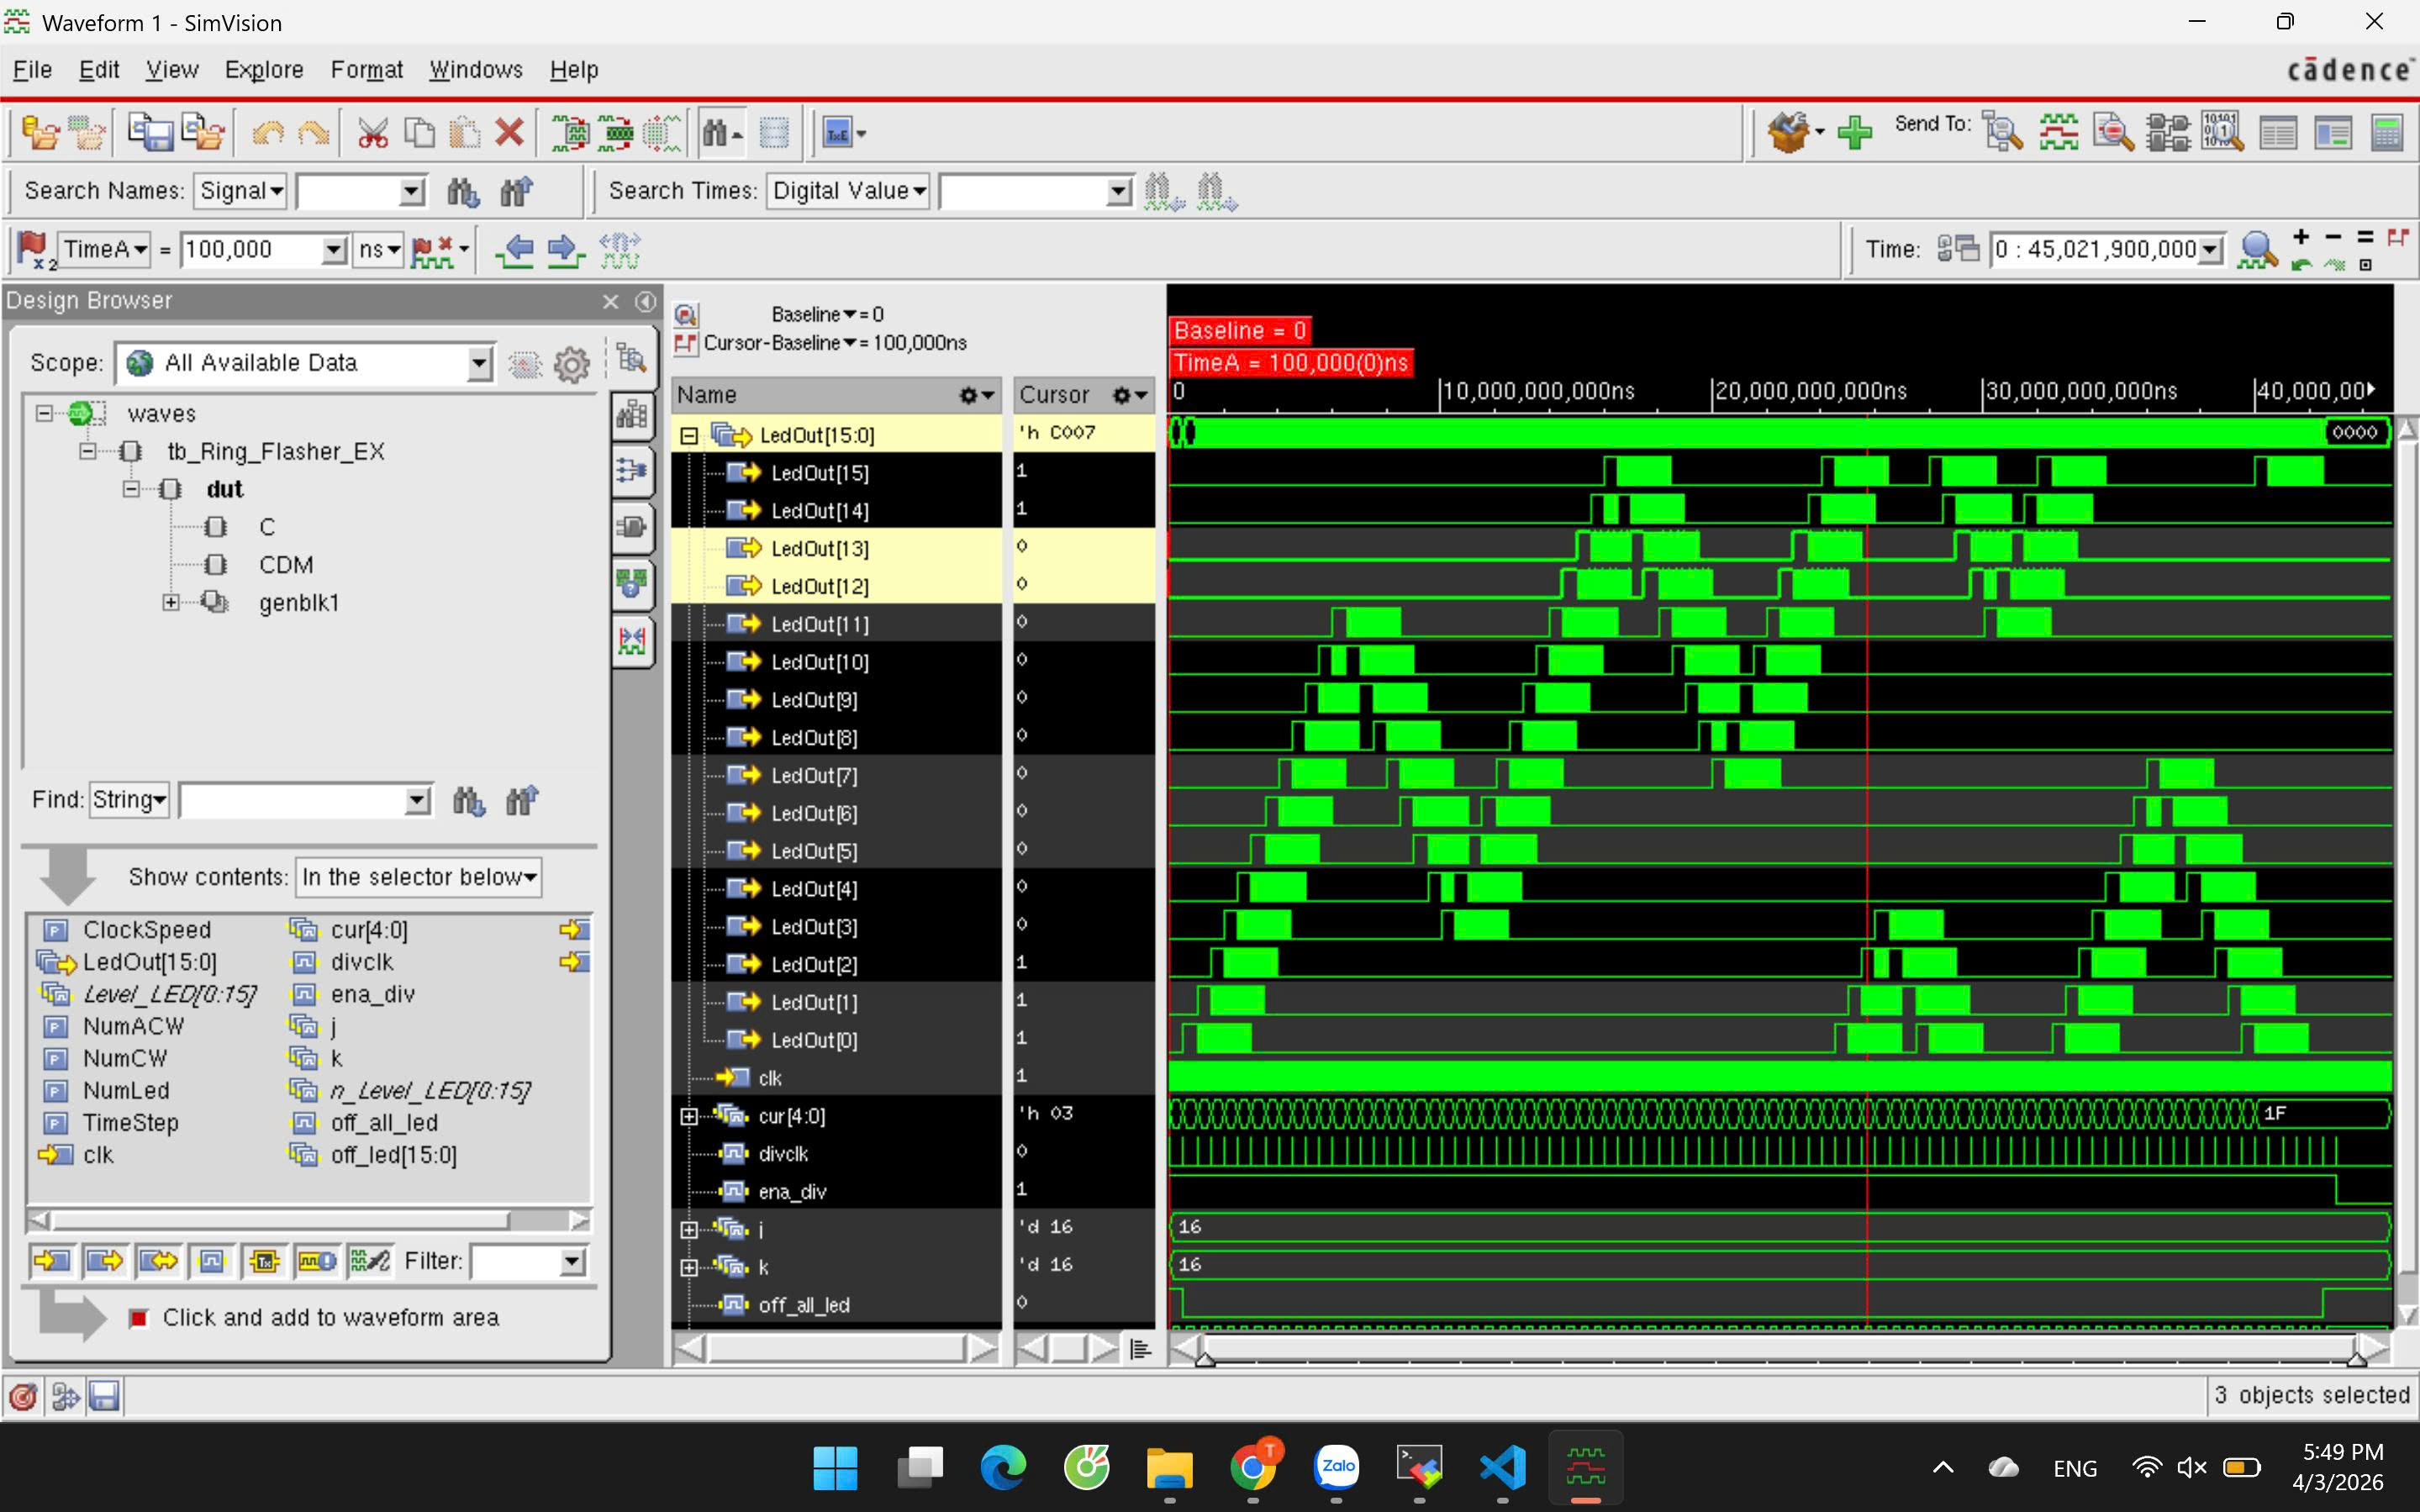
\includegraphics[width=1\linewidth]{graphics/TC1_Normal_Operation.jpg}
    \caption{Waveform of TC1: Normal Operation - shows continuous CW/ACW sequence with cycle completion before fade-out and IDLE transition.}
\end{figure}

\begin{figure}[H]
    \centering
    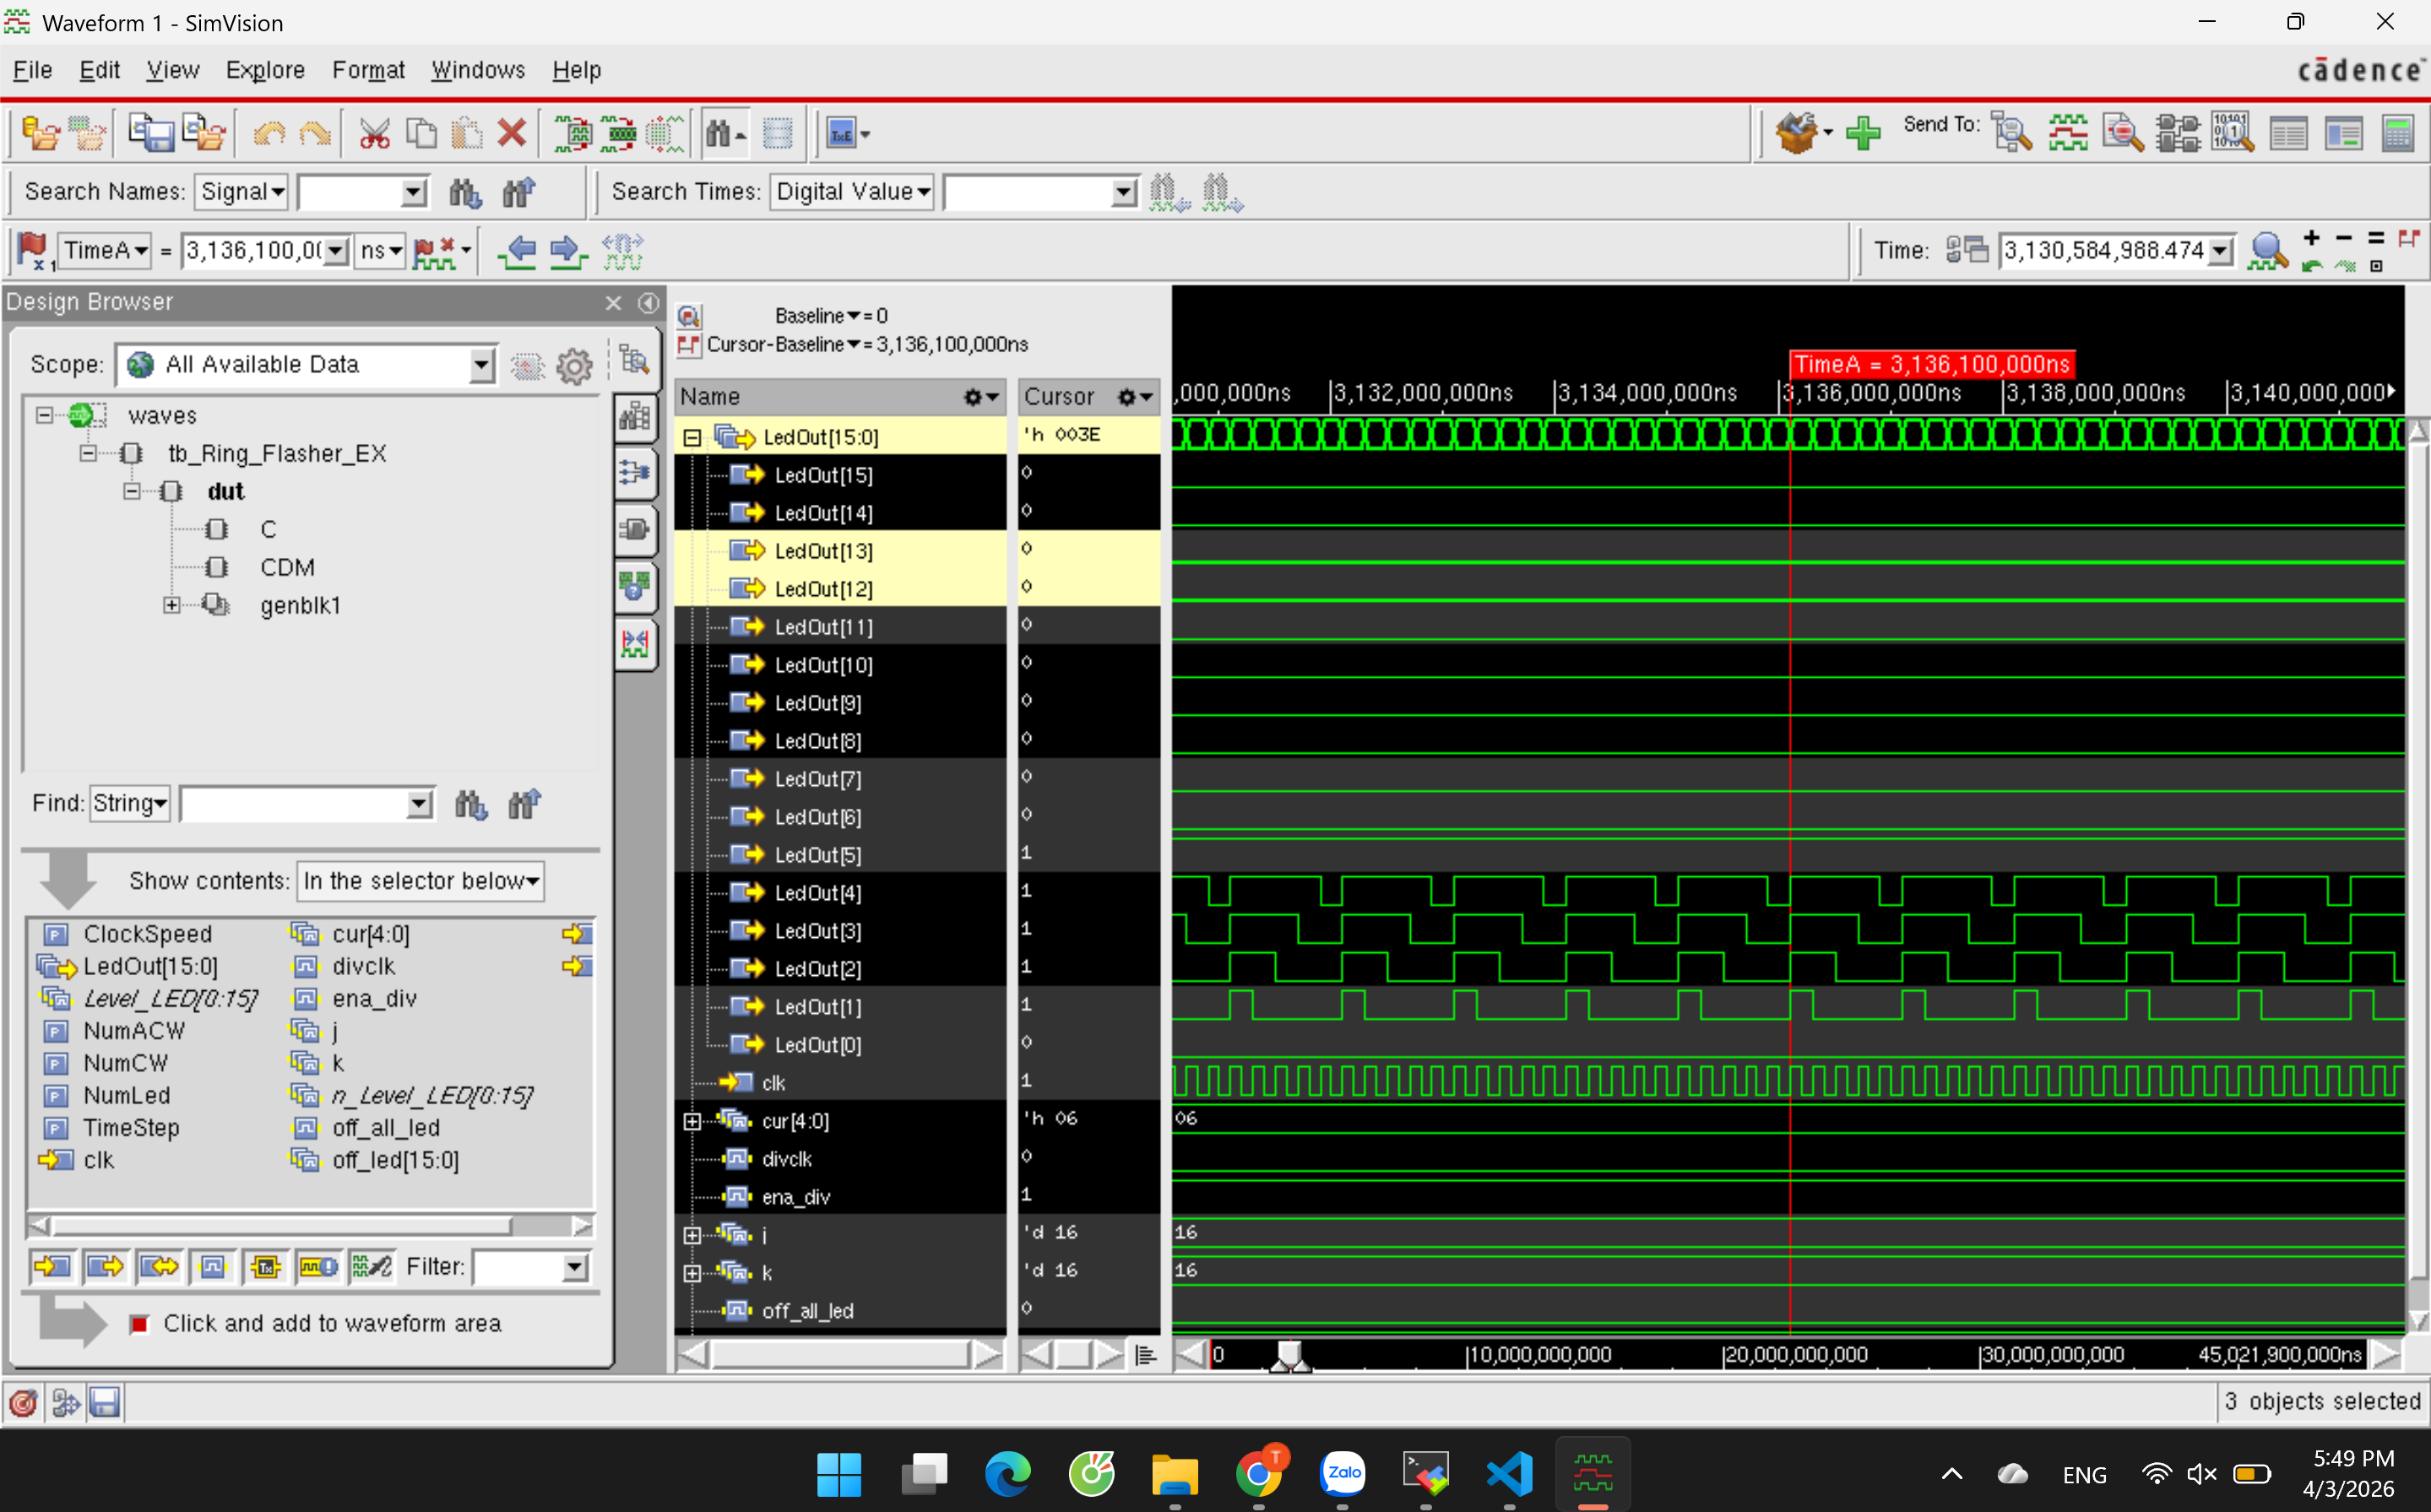
\includegraphics[width=1\linewidth]{graphics/TC1_Normal_Operation1.png}
    \caption{Zoomed waveform of TC1: Fade-Out - demonstrates brightness decrementing on each \texttt{divclk}.}
\end{figure}
\subsubsection{TC2: Mid-cycle Rep-off Test}

\textbf{Objective}: Verify the ring flasher behavior when \texttt{rep} is deasserted mid-cycle, including the one-divclk delay before the first bright state.

\textbf{Test Flow}:
\begin{enumerate}
    \item Apply reset
    \item Set \texttt{rep = 1} and observe the first active transition after one divided-clock pulse
    \item Keep \texttt{rep = 1} long enough for the FSM to complete one full upward ring sequence
    \item Set \texttt{rep = 0} during operation and observe that fade-out starts only after the current upward cycle finishes
\end{enumerate}

\textbf{Expected Behavior}:
\begin{itemize}
    \item After \texttt{rep = 1} is asserted, the FSM waits for one \texttt{divclk} pulse before entering the first bright state
    \item LED sequence begins from the initial state and performs the full upward run before any fade-out action
    \item If \texttt{rep} goes low mid-cycle, the FSM does not fade out immediately
    \item The design finishes the current upward ring movement, then transitions to OFF\_STATE and fades out
    \item After brightness reaches zero, the FSM returns to the initial IDLE state
    \item Confirms the intended delayed start and deferred fade-out behavior of the controller
\end{itemize}

\begin{figure}[H]
    \centering
    % Place waveform image for TC2 here.
    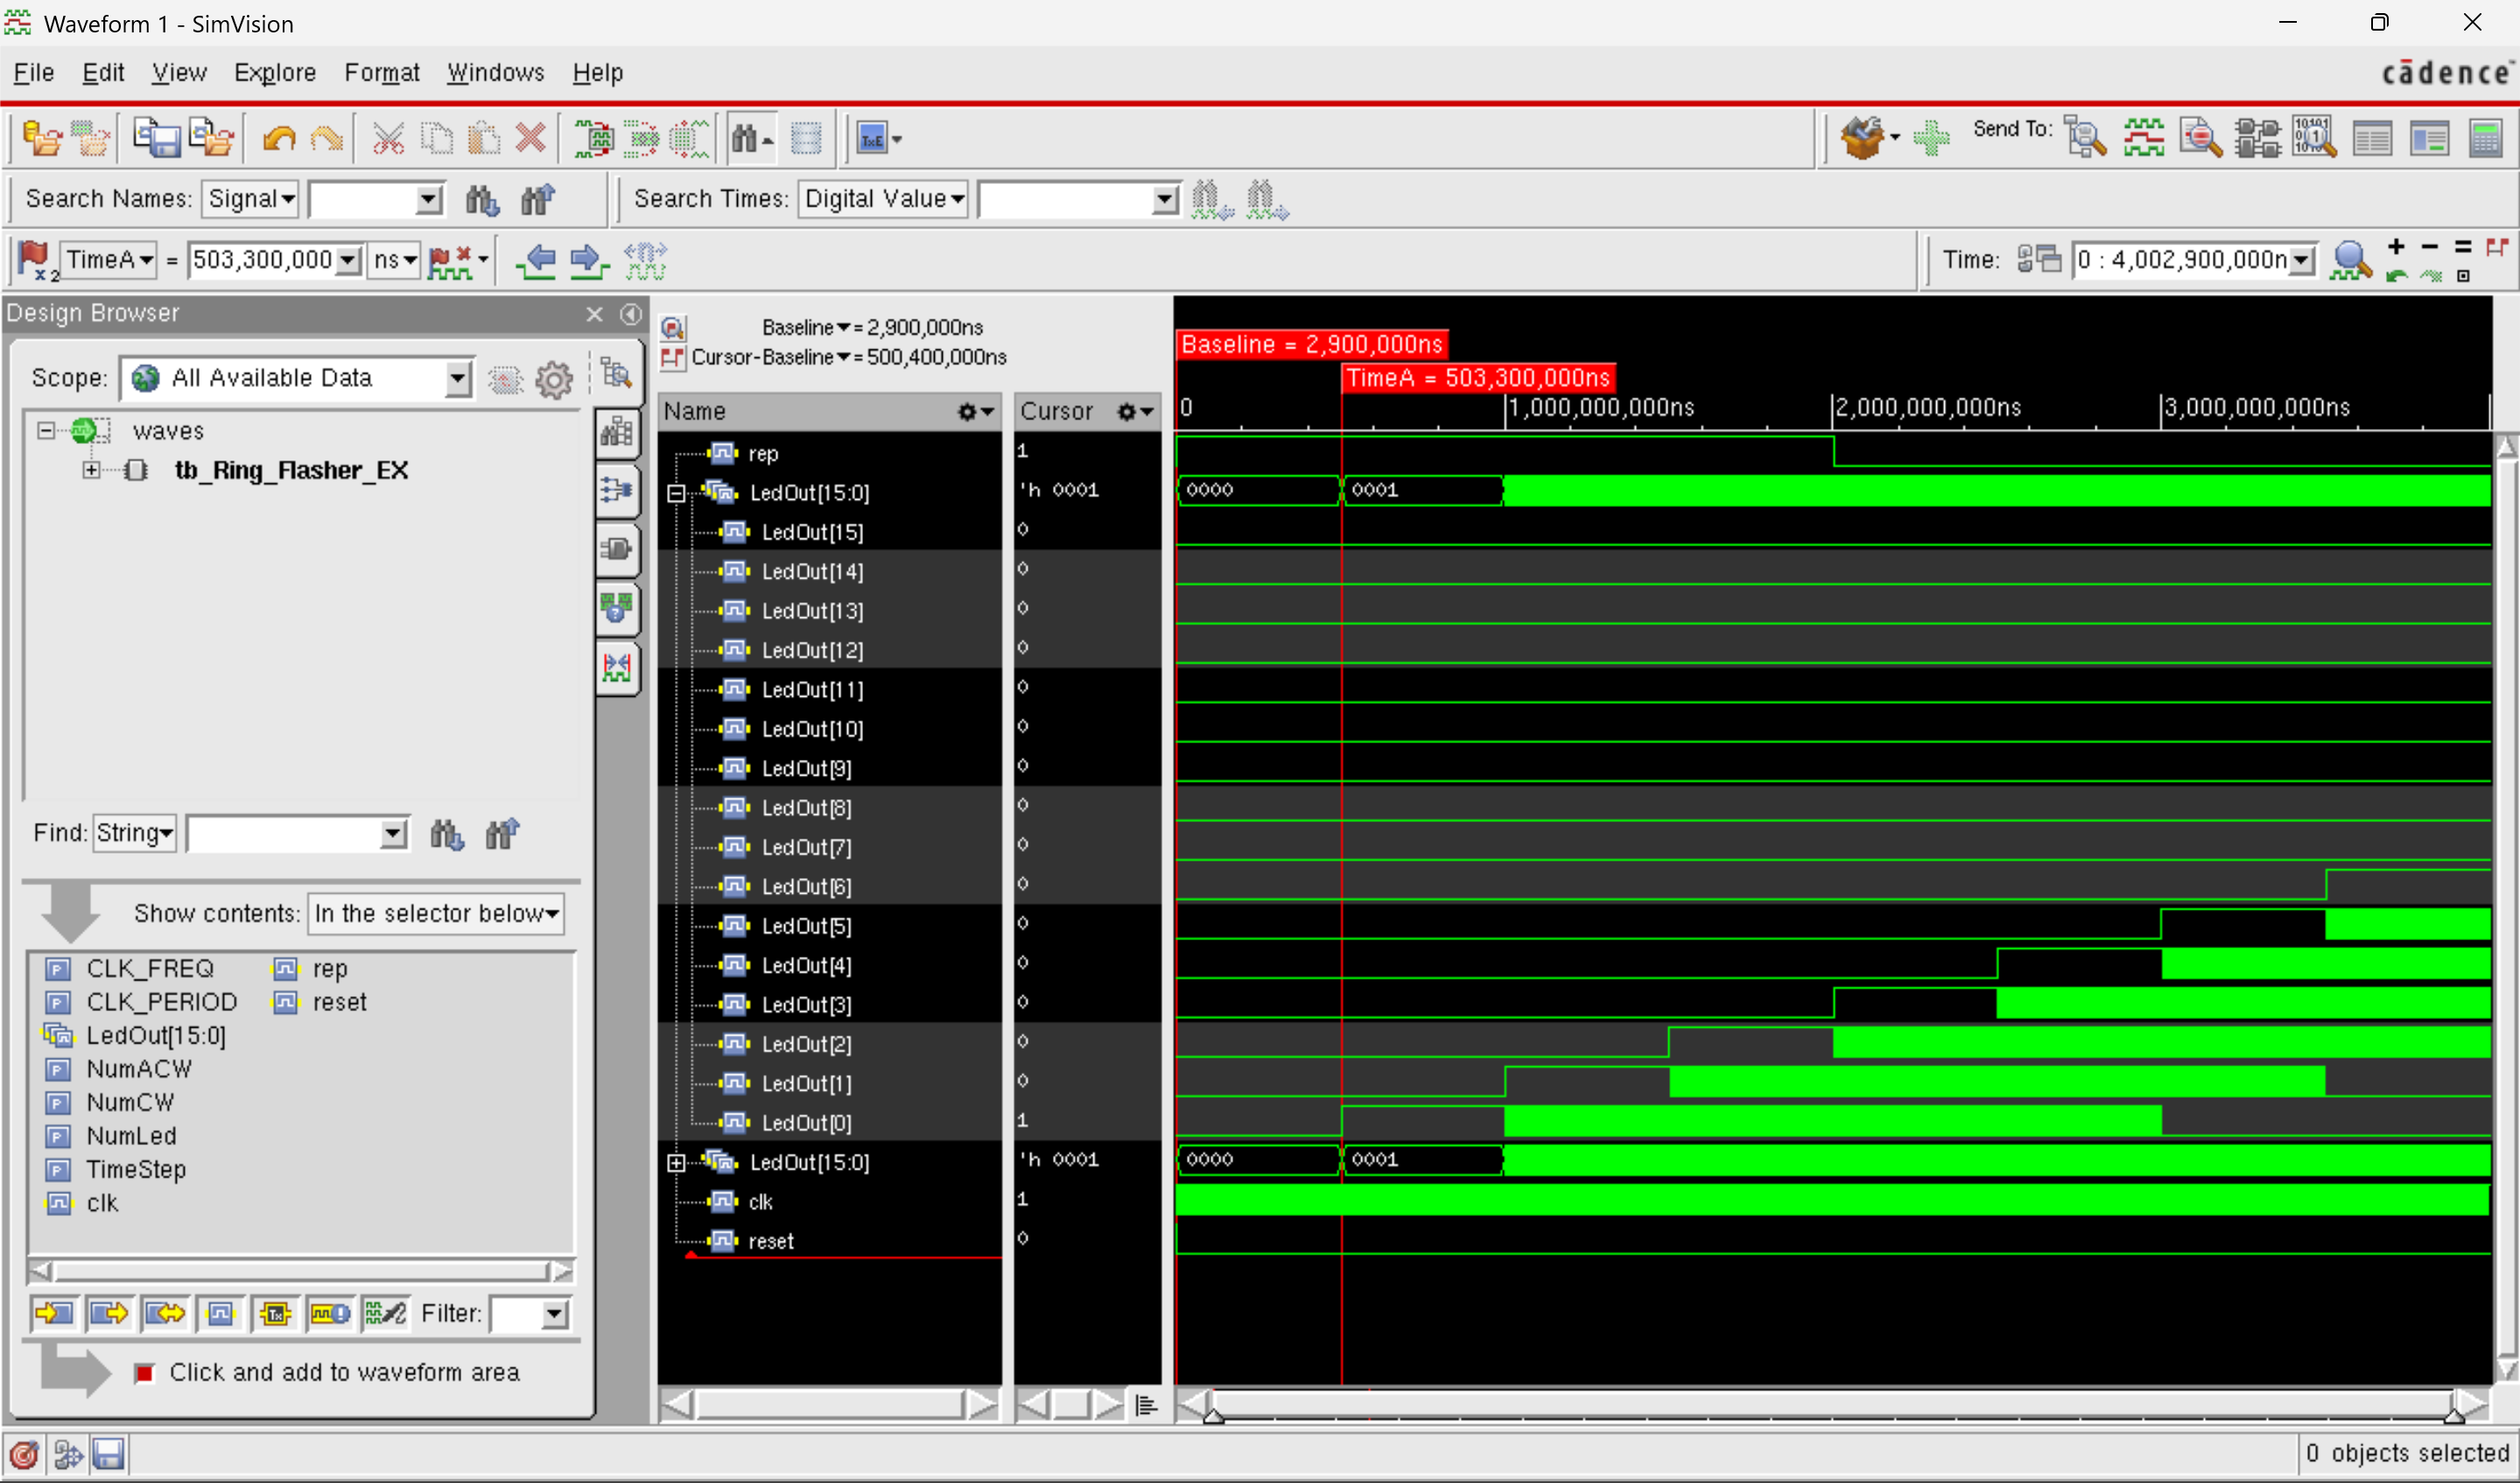
\includegraphics[width=1\linewidth]{graphics/TC2.png}
    \caption{Waveform of TC2: Mid-cycle rep-off behavior - demonstrates the delayed start, completion of the upward sequence, and deferred fade-out.}
\end{figure}

\subsubsection{TC3: Mid-run Reset Test}

\textbf{Objective}: Verify that asserting reset in the middle of operation stops the system immediately and returns it to the initial state.

\textbf{Test Flow}:
\begin{enumerate}
    \item Apply reset
    \item Set \texttt{rep = 1} and let the sequence run normally
    \item Assert \texttt{reset = 1} in the middle of the sequence
    \item Release reset and observe the system return to the initial state
    \item Re-apply \texttt{rep = 1} if needed to confirm restart from the beginning
\end{enumerate}

\textbf{Expected Behavior}:
\begin{itemize}
    \item When \texttt{reset} is asserted, all outputs stop immediately without waiting for the current cycle to finish
    \item LED activity is cleared at once and the FSM returns to the initial state
    \item After reset release, the controller remains in IDLE until \texttt{rep} is asserted again
    \item Confirms that reset has higher priority than the normal fade-out path
    \item Validates immediate termination behavior when reset is toggled during operation
\end{itemize}

\begin{figure}[H]
    \centering
    % Place waveform image for TC3 here.
    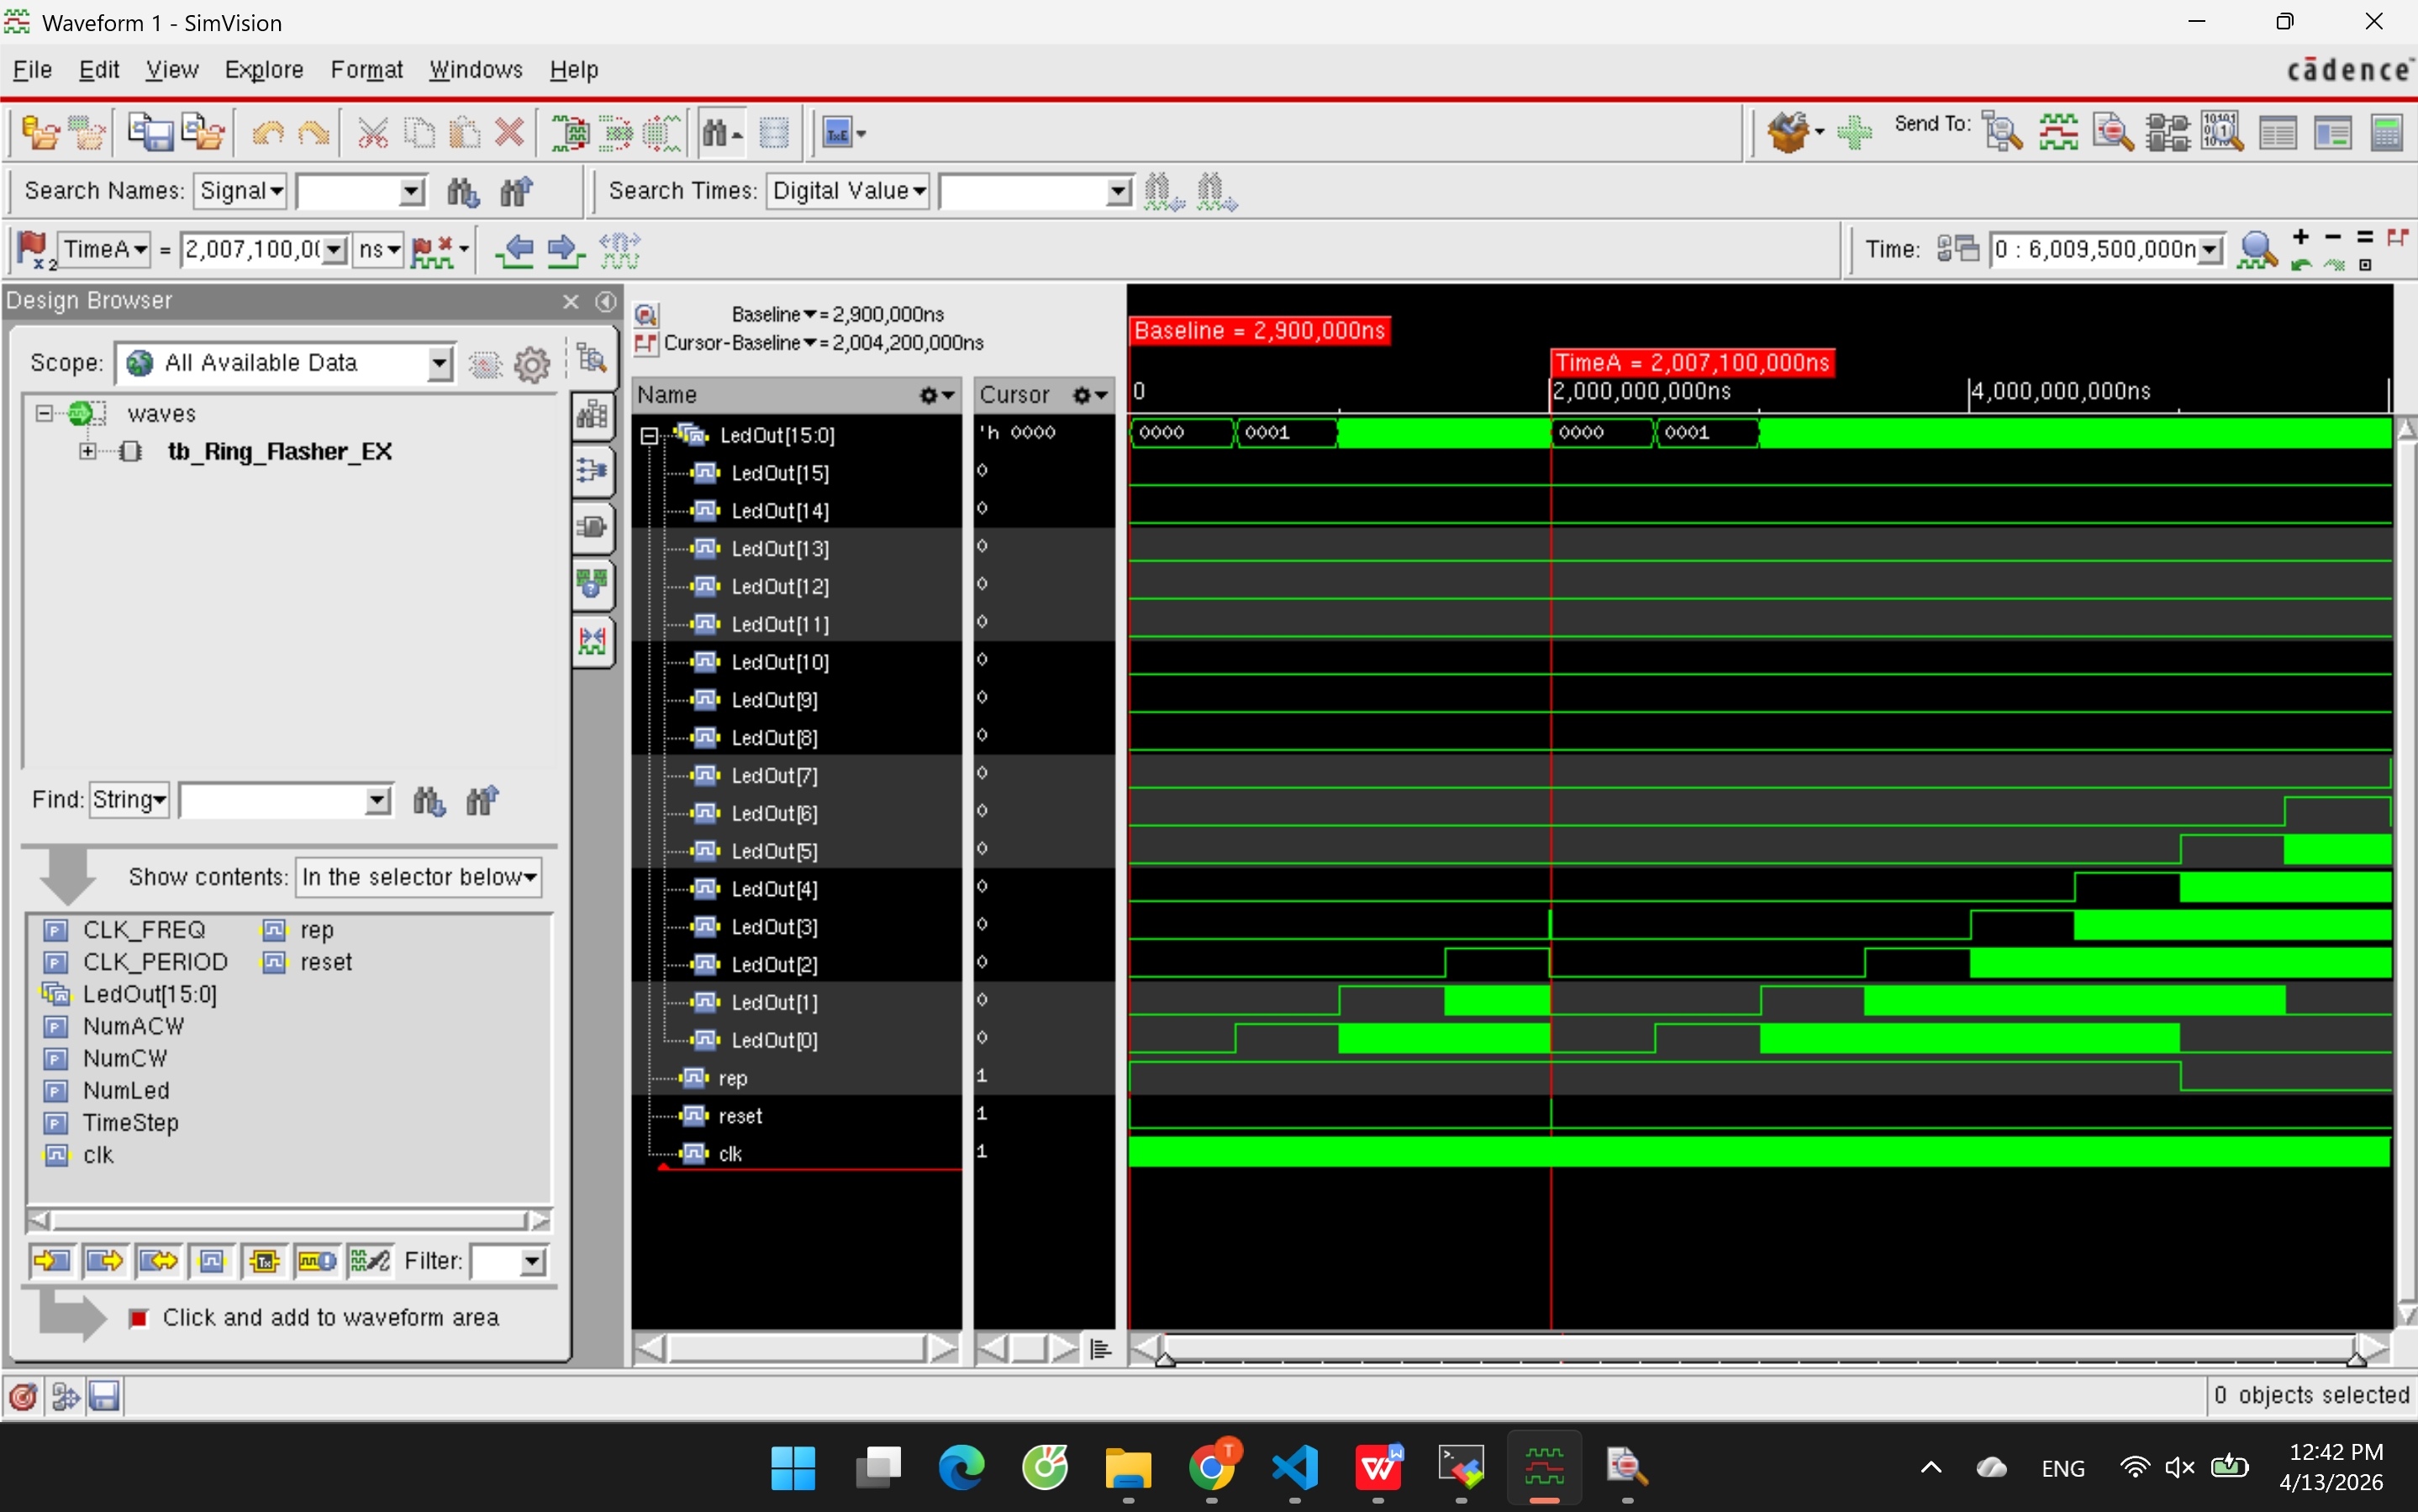
\includegraphics[width=1\linewidth]{graphics/TC3.png}
    \caption{Waveform of TC3: Mid-run reset behavior - demonstrates immediate stop and return to the initial state.}
\end{figure}

\subsection{Simulation Results Summary}

The comprehensive testbench validates the following functional areas:

\begin{itemize}[leftmargin=*, labelsep=0.5cm]
    \item \textbf{State Machine Correctness}: All four states (IDLE, CW, ACW, OFF) transition according to FSM specification and input conditions.
    
    \item \textbf{Sequence Timing}: CW and ACW sequences execute for exactly 12 and 8 steps respectively, with transitions synchronized to \texttt{divclk}.
    
    \item \textbf{Brightness Control}: PWM duty cycles correctly implement 6 brightness levels (0--5) with proper decay during fade-out.
    
    \item \textbf{Reset Functionality}: Reset immediately clears the active operation and returns the system to a clean initial condition.
    
    \item \textbf{Feedback Control}: The \texttt{off\_all} signal correctly detects when all LEDs have faded and triggers FSM state transition.
    
    \item \textbf{Clock Divider Stability}: Divider maintains consistent timing across extended operations without drift or overflow.
\end{itemize}

These three test cases cover the normal operation, deferred fade-out after a mid-cycle \texttt{rep} change, and immediate shutdown on reset, demonstrating that the Ring Flasher design meets its functional and timing specifications.